
\newcommand{\degree}{\ensuremath{^{\circ}}}

\chapter{Kreslenie molekuly}

Po tom co ziskame a aplikujeme mapovanie medzi sablonovou a cielovou molekulou RNA,
ziskame cielovu molekulu s ciastocnou vizualizaciou, ktorej zvysok treba dopocitat.

Po operaciach delete ostavaju v molekule prazdne diery, naopak po insertoch potrebujeme
vypocitat, kam umiestnime bazovy par, resp. samotnu bazu, pripadne este potrebujeme pre
nu urobit miesto. Update vrcholu v strome nerobi ziadne strukturne zmeny, zmeni sa iba
nazov bazy na danom mieste.

Sekundarna struktura RNA obsahuje mnozstvo motivov popisanych na obrazku \ref{obr:RNA_motifs}.
Vo vseobecnosti ale sa kazdy z tychto motivov sklada zo stemu a loopu.

Stemom budeme dalej nazyvat cast RNA ktora zodpoveda vnutornemu vrcholu v strome. Loop
budeme oznacovat listy v RNA strome (lese), nezalezi ci je to bulge, interior loop, hairpin
alebo multibranch loop, ako aj ukazuje obrazok \ref{obr:RNA_motifs_stem_loop}.

Stem zacina vzdy v najvyssom vrchole stromu (v smere ku korenu), ktory je zaroven vnutornym
vrcholom a nema ziadnych surodencov, ktory by boli rovnako vnutornymi vrcholmi.
To znamena, ze do multibranch loop vchadza 1 stem (ten tu konci) a vychadza z nej niekolko novych stemov.
Naopak pre bulge a interior loop jeden stem vchadza do struktury ale pokracuje dalej.

\begin{figure}[H]
\centering
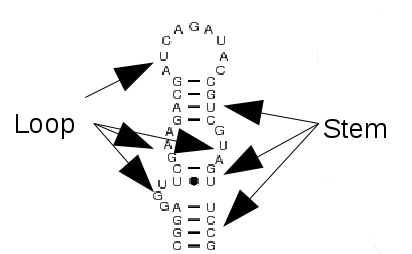
\includegraphics[width=50mm, height=35mm]{../img/struktury_v_rna-stem_loop.png}
%TODO klasicky obrazok RNA molekuly, v ktorej farbami odlisim stem a loop.
\caption{Stem a loop v molekule}
\label{obr:RNA_motifs_stem_loop}
\end{figure}

\section{Struktury RNA}

V clanku od \citet{RNA_DRAW} autori popisuju pravidla vizualizacie sekundarnej struktury RNA.

Nakreslenie musi byt rovinne bez krizeni, bazy tvoriace rozne druhy loopov musia leziat na kruzniciach
a bazy tvoriace stem maju lezat na priamke.
Dalsim pravidlom je, ze vzdialenost medzi bazami ma byt konstantna, ci uz vzdialenost medzi bazami jedneho paru,
alebo bazami sekvencie.

Ako je ukazane na obrazku \ref{obr:RNA_full}, pravidla niesu niekedy respektovane. To ztazuje pouzitie obrazka
ako sablony, kedze vo vyslednom obrazku chceme vsetky tieto pravidla respektovat.

\section{Algoritmus}

Ciastocnej vizualizacie ktoru dostavame z mapovania sa chceme dotykat co najmenej. To znamena,
ze vsetky zasahy sa snazime robit iba v miestach, ktore boli dotknute vkladanim alebo mazanim baz.

Jedine vynimky su normalizacia vzdialensoti medzi bazovymi parmi a vyrovnavanie stemov.

\subsection{Normalizácia vzdialeností v bázových pároch a vyrovnavanie stemov}

Ako bolo uvedene, stemom rozumieme nevetviacu sa cast stromu tvorenu iba bazovymi parmi.

Algoritmus normalizácie vzdialeností medzi vrcholmi bázových párov stojí iba v preiterovani celeho stromu
a ak nejake parove vrcholy su od seba priliz vzdialene, priblizi ich k sebe.

Vyrovnavaci algoritmus prechadza vsetky stemy. Z ich zaciatkov vedie priamku na ktorej maju byt podla pravidla ulozene
vsetky stemove vrcholy. Rotaciami a posunutiami podstromov vieme docielit to, aby vrcholy stemu na tejto priamke lezali.

% TODO obrazok vyrovnavania

\subsection{Operacie na stromoch}

Citatela zoznamime s 2 operaciami, ktore budeme vykonavat na molekule. Tie budeme pouzivat nezavisle
na tom, ci vrcholy do stromu vkladame alebo mazeme.

\begin{algorithm}
  \caption{Rozlozenie baz na kruznicu}
  \label{alg:operacia_circle_reinsert}
  \begin{algorithmic}[1]
    \Procedure {rozlozBazy}{Begin, End, Bases}
      \State $n \gets$ velkost zoznamu baz $Bases$
      \State $\Gamma \gets$ dostatocne velka kruznica pre $n$ bodov prechadzajuca bodmi $Begin$ a $End$
      \State $\Pi \gets$ rozdel kruhovy obluk kruznice $\Gamma$ od $Begin$ po $End$ na $n$ bodov
      \ForAll{$i$ in 1 .. $n$}
        \State nastav poziciu bazy $Bases[i]$ na bod $\Pi[i]$
      \EndFor
    \EndProcedure
  \end{algorithmic}
\end{algorithm}

\begin{algorithm}
  \caption{Posunutie podstromu}
  \label{alg:operacia_tree_shift}
  \begin{algorithmic}[1]
    \Procedure {posunPodstrom}{Root, Vector}
      \ForAll {vrchol $V$ v podstrome vrcholu $Root$}
        \If {vrchol $V$ uz ma urcenu poziciu, t.j. nieje prave vlozeny}
          \State pripocitaj k pozicii bazy $V$ vektor $Vector$
        \EndIf
      \EndFor
    \EndProcedure
  \end{algorithmic}
\end{algorithm}

Ako sme pisali uz skor, vsetky loop struktury maju byt ulozene na kruzniciach. K tomu nam pomoze funkcia
\ref{alg:operacia_circle_reinsert}. Ta dostava na vstupe zoznam baz $Bases$ a dva body v rovine, $Begin$ a $End$.
Tymito bodmi potrebujeme viest kruznicu, ktora bude dostatocne velka, teda aby na nu vsetky bazy zo zoznamu vosli.
Velkostou kruznice v tomto pripade myslime dlzku kruhoveho obluku medzi vrcholmi $Begin$ a $End$.

V nasom programe pouzivame iteracny algoritmus, ktory ju pomaly zvacsuje alebo zmensuje.
Nakoniec bud najde kruznicu ktorej velkost je optimalna, alebo ani na maximalny pocet krokov taku kruznicu nenajde
a tak vrati tu z posledneho kroku.
% TODO obrazok iterovania zvacsovania kruznice

Operacia v ramci algoritmu \ref{alg:operacia_tree_shift} nam pomoze urobit miesto na novo vlozene bazove pary,
alebo naopak ak sme nieco zmazali, tak dokaze cely podstrom pritiahnut spat.

\subsection{Vkladanie noveho vrcholu do stromu}

Pri vkladani noveho vrcholu do stromu mozu nastat nasledovne moznosti.

Ak vkladame list do hairpinu, je to jednoduche, potrebujeme iba pouzit proceduru z algoritmu \ref{alg:operacia_circle_reinsert}
s parametrami $Begin = $ pozicia prvej bazy z bazoveho paru, $End = $ pozicia druhej bazy z paru
a $Bases = $ zoznam vsetkych potomkov.

Trochu zlozitejsie je to pri vkladani listu do stemu. V tomto pripade bud uz stem obsahoval nejaky loop, alebo vznika nova.
Najprv potrebujeme upravit vzdialenost medzi vrcholmi stemu, teda posunut cely podstrom aby nam dane bazy vosli.
To vyriesime algoritmom \ref{alg:operacia_tree_shift}. Nasledne najdeme kruznicu a bazy na nu naukladame.

Vkladanie bazoveho paru do stemu je jednoduche. Najprv posunieme cely podstrom a urobime tak miesto pre novu dvojicu
baz, a potom ich ulozime na poziciu kde by mala patrit. Moze sa stat, ze vlozenim vrcholu do stemu zdedime niekolko
listov z predka. V tomto pripade iba pouzijeme operaciu vlozenia vrcholu a updatu loopov pred aj za vlozenym vrcholom.

\subsection{Modifikacia multibrach loop}

Modifikacia multibranch loop je zlozitejsia ako vsetky predchadzajuce pripady. Obrazky su vacsinou rucne upravene tak,
aby bol co najkompaktnejsi a kvoli tomu sa casto nerespektuju pravidla o kruznicovom tvare struktury.
Kvoli tomu sa snazime do tejto struktury nezasahovat, ak sa to da.

Prekresleniu celej struktury sa mozeme vyhnut napriklad pri zmene poctu listov medzi jednotlivymi vetvami.
Ak je zmena dostatocne mala, mozeme vrcholy roztiahnut, alebo naopak priblizit k sebe.

Ak sa jedna o pridanie/odobratie celej vetvy stromu, modifikacii sa nevyhneme. V tom pripade potrebujeme
rozdistribuovat vsetky vrcholy patriace do loop na kruznicu. Je to podobny proces ako sa pouziva iba pre samotne loopy,
ale potrebujeme posuvat cele podstromy a zrotovat ich spravnym smerom.

\subsection{Mazanie vrcholu zo stromu}

Mazanie povazujeme za inverznu operaciu voci vkladaniu do stromu. Vzhladom k tomu, pouzivame rovnake operacie
rozdistribuovania vrcholov v loope, alebo posuvanie podstromu, ktore sa deje v tomto pripade opacnym smerom
k predkovi.




